%package list
\documentclass{article}
\usepackage[top=3cm, bottom=3cm, outer=3cm, inner=3cm]{geometry}
\usepackage{multicol}
\usepackage{graphicx}
\usepackage{url}
%\usepackage{cite}
\usepackage{hyperref}
\usepackage{array}
%\usepackage{multicol}
\newcolumntype{x}[1]{>{\centering\arraybackslash\hspace{0pt}}p{#1}}
\usepackage{natbib}
\usepackage{pdfpages}
\usepackage{multirow}
\usepackage[normalem]{ulem}
\useunder{\uline}{\ul}{}
\usepackage{svg}
\usepackage{xcolor}
\usepackage{listings}
\lstdefinestyle{ascii-tree}{
	literate={├}{|}1 {─}{--}1 {└}{+}1 
}
\lstset{basicstyle=\ttfamily,
	showstringspaces=false,
	commentstyle=\color{red},
	keywordstyle=\color{blue}
}
%\usepackage{booktabs}
\usepackage{caption}
\usepackage{subcaption}
\usepackage{float}
\usepackage{array}

\newcolumntype{M}[1]{>{\centering\arraybackslash}m{#1}}
\newcolumntype{N}{@{}m{0pt}@{}}


%%%%%%%%%%%%%%%%%%%%%%%%%%%%%%%%%%%%%%%%%%%%%%%%%%%%%%%%%%%%%%%%%%%%%%%%%%%%
%%%%%%%%%%%%%%%%%%%%%%%%%%%%%%%%%%%%%%%%%%%%%%%%%%%%%%%%%%%%%%%%%%%%%%%%%%%%
\newcommand{\itemEmail}{aalfonso@unsa.edu.pe}
\newcommand{\itemStudent}{Repositorio: proyecto}
\newcommand{\itemCourse}{PWEB 2}
\newcommand{\itemCourseCode}{20220596}
\newcommand{\itemSemester}{I}
\newcommand{\itemUniversity}{Universidad Nacional de San Agustín de Arequipa}
\newcommand{\itemFaculty}{Facultad de Ingeniería de Producción y Servicios}
\newcommand{\itemDepartment}{Departamento Académico de Ingeniería de Sistemas e Informática}
\newcommand{\itemSchool}{Escuela Profesional de Ingeniería de Sistemas}
\newcommand{\itemAcademic}{2023 - A}
\newcommand{\itemInput}{Del 29 Junio 2023}
\newcommand{\itemOutput}{Al 14 Julio 2023}
\newcommand{\itemPracticeNumber}{07}
\newcommand{\itemTheme}{Relaciones de uno a muchos, muchos a muchos y impresion de pdf y emails}
%%%%%%%%%%%%%%%%%%%%%%%%%%%%%%%%%%%%%%%%%%%%%%%%%%%%%%%%%%%%%%%%%%%%%%%%%%%%
%%%%%%%%%%%%%%%%%%%%%%%%%%%%%%%%%%%%%%%%%%%%%%%%%%%%%%%%%%%%%%%%%%%%%%%%%%%%

\usepackage[english,spanish]{babel}
\usepackage[utf8]{inputenc}
\AtBeginDocument{\selectlanguage{spanish}}
\renewcommand{\figurename}{Figura}
\renewcommand{\refname}{Referencias}
\renewcommand{\tablename}{Tabla} %esto no funciona cuando se usa babel
\AtBeginDocument{%
	\renewcommand\tablename{Tabla}
}

\usepackage{fancyhdr}
\pagestyle{fancy}
\fancyhf{}
\setlength{\headheight}{30pt}
\renewcommand{\headrulewidth}{1pt}
\renewcommand{\footrulewidth}{1pt}
\fancyhead[L]{\raisebox{-0.2\height}{
\includegraphics[width=3cm]{img/logo_episunsa.png}}}
\fancyhead[C]{\fontsize{7}{7}\selectfont	\itemUniversity \\ \itemFaculty \\ \itemDepartment \\ \itemSchool \\ \textbf{\itemCourse}}
\fancyhead[R]{\raisebox{-0.2\height}{
\includegraphics[width=1.2cm]{img/logo_abet}}}
\fancyfoot[L]{Grupo: Seb . Klis . Maxs. Mau}
\fancyfoot[C]{\itemCourse}
\fancyfoot[R]{Página \thepage}

% para el codigo fuente
\usepackage{listings}
\usepackage{color, colortbl}
\definecolor{dkgreen}{rgb}{0,0.6,0}
\definecolor{gray}{rgb}{0.5,0.5,0.5}
\definecolor{mauve}{rgb}{0.58,0,0.82}
\definecolor{codebackground}{rgb}{0.95, 0.95, 0.92}
\definecolor{tablebackground}{rgb}{0.8, 0, 0}

\lstset{frame=tb,
	language=bash,
	aboveskip=3mm,
	belowskip=3mm,
	showstringspaces=false,
	columns=flexible,
	basicstyle={\small\ttfamily},
	numbers=none,
	numberstyle=\tiny\color{gray},
	keywordstyle=\color{blue},
	commentstyle=\color{dkgreen},
	stringstyle=\color{mauve},
	breaklines=true,
	breakatwhitespace=true,
	tabsize=3,
	backgroundcolor= \color{codebackground},
}

\begin{document}
	
	\vspace*{10px}

\begin{center}	
	\fontsize{17}{17} \textbf{ Informe de Laboratorio 05}
\end{center}
\centerline{\textbf{\Large Tema: Django}}
%\vspace*{0.5cm}	

\begin{flushright}
	\begin{tabular}{|M{2.5cm}|N|}
		\hline 
		\rowcolor{tablebackground}
		\color{white} \textbf{Nota}  \\
		\hline 
		\\[30pt]
		\hline 			
	\end{tabular}
\end{flushright}	

\begin{table}[H]
	\begin{tabular}{|x{4.7cm}|x{4.8cm}|x{4.8cm}|}
		\hline 
		\rowcolor{tablebackground}
		\color{white} \textbf{Estudiantes} & \color{white}\textbf{Escuela}  & \color{white}\textbf{Asignatura}   \\
		\hline 
		{- Alejandro Sebastian Alfonso Huacasi \par aalfonso@unsa.edu.pe \par - Klismann Chancuaña Alvis \par kchancuana@unsa.edu.pe \par - Mauricio Elias Congona Manrique \par mcongonam@unsa.edu.pe \par - Maxs Sebastian Joaquin Forocca Mamani \par mforocca@unsa.edu.pe } & Escuela Profesional de Ingenieria de Sistemas & {Programación web 2 \par Semestre: A}     \\
		\hline 			
	\end{tabular}
\end{table}		

\begin{table}[H]
	\begin{tabular}{|x{4.7cm}|x{4.8cm}|x{4.8cm}|}
		\hline 
		\rowcolor{tablebackground}
		\color{white}\textbf{Laboratorio} & \color{white}\textbf{Tema}  & \color{white}\textbf{Duración}   \\
		\hline 
		05 & Django & 04 horas   \\
		\hline 
	\end{tabular}
\end{table}

\begin{table}[H]
	\begin{tabular}{|x{4.7cm}|x{4.8cm}|x{4.8cm}|}
		\hline 
		\rowcolor{tablebackground}
		\color{white}\textbf{Semestre académico:} & \color{white}\textbf{Fecha de inicio}  & \color{white}\textbf{Fecha de entrega}   \\
		\hline 
		2023 - A & Del 26 Junio 2023 &  Al 03 Julio 2023  \\
		\hline 
	\end{tabular}
\end{table}
	
	TAREA
\begin{itemize}		
	\item Integrar los conocimientos adquiridos en el curso
        \item Trabajar en equipo
        \item Desarrollar una aplicación Web para una empresa real, que incluya: Backend (Django) y FrontEnd (Ajax / Framework JavaScript: Angular)
\end{itemize}

		
	\section{Equipos, materiales y temas utilizados}
\begin{itemize}
	\item Sistema Operativo (GNU/Linux de preferencia).
	\item GNU Vim.
	\item Python 3
	\item Git.
	\item Cuenta en GitHub con el correo institucional.
        \item Ajax
        \item Django 4
        \item JavaScript
        \item Angular
\end{itemize}
	
	\section{URL de Repositorio Github del modelo de latex para los informes}
\begin{itemize}
	\item URL del Repositorio GitHub para clonar o recuperar.
	\item \url{https://github.com/rescobedoq/programacion.git}
	\item URL para el laboratorio 01 en el Repositorio GitHub.
	\item \url{https://github.com/rescobedoq/programacion/tree/main/lab01}
\end{itemize}
	
	\section{Actividades con el repositorio GitHub}

\subsection{Creando e inicializando repositorio GitHub}
\begin{itemize}	
	\item Como ya tenemos nuestro repositorio GitHub y además esta clonado e inicializado en nuestra máquina local.
	\item Se realizaron los siguientes comandos en la computadora:
\end{itemize}	

\begin{lstlisting}[language=bash,caption={Creando carpeta de trabajo dentro de nuestro repositorio clonado en mi maquina local}][H]
	$ cd Pweb2-Lab-B
   $ mkdir ProyectoFinal
\end{lstlisting}
\begin{lstlisting}[language=bash,caption={Dirijíéndonos a la carpeta de trabajo}][H]
	$ cd ProyectoFinal
\end{lstlisting}	
\subsection{Commits}
\begin{itemize}	
	\item A continucación se mostraran capturas de los commits:
\end{itemize}	
\begin{figure}[H]
	\centering
	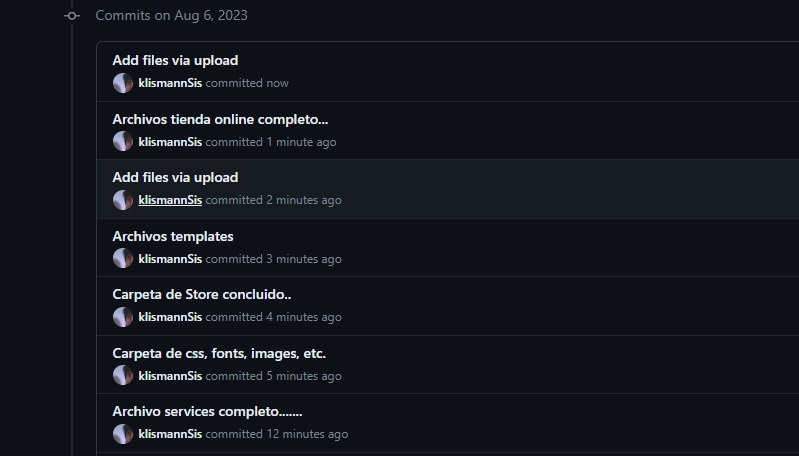
\includegraphics[width=0.8\textwidth,keepaspectratio]{img/imagen11.jpg}
	%\includesvg{img/automata.svg}
	%\label{img:mot2}
	%\caption{Product backlog.}
\end{figure}
\begin{figure}[H]
	\centering
	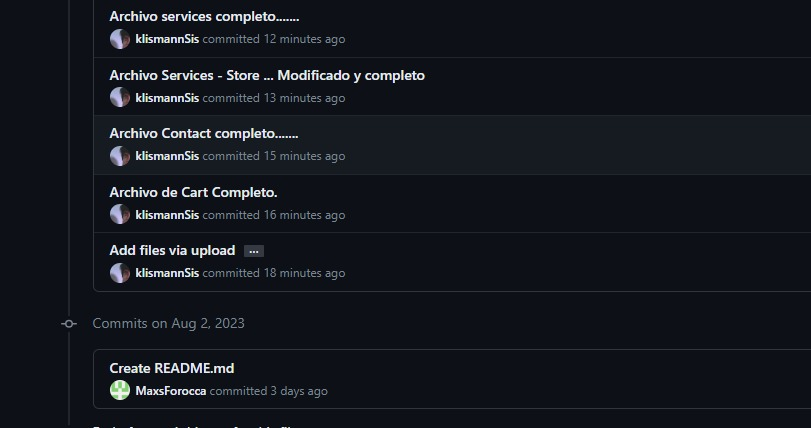
\includegraphics[width=0.8\textwidth,keepaspectratio]{img/imagen12.jpg}
	%\includesvg{img/automata.svg}
	%\label{img:mot2}
	%\caption{Product backlog.}
\end{figure}
\begin{itemize}	
	\item Explicaremos algunos archivos de nuestro proyecto final:
\end{itemize}	
\lstinputlisting[language=Python, caption={apps.py, se encuentra en la carpeta tiendaOnline, dentro de la carpeta de cart},numbers=left,]{src/apps.py}
\begin{itemize}
        \item from django.apps import AppConfig: Esta línea importa la clase AppConfig del módulo django.apps. AppConfig es una clase de Django que se utiliza para configurar y personalizar la aplicación.
        \item class CartConfig(AppConfig):: Aquí defines una nueva clase llamada CartConfig que hereda de AppConfig. Esto significa que estás creando una configuración personalizada para una parte específica de tu aplicación.
        \item defaultautofield = 'django.db.models.BigAutoField': Estableces el campo automático predeterminado que se utilizará para las claves primarias en los modelos de esta aplicación. En este caso, estás utilizando un campo llamado BigAutoField, que es una variante de clave primaria automática que admite valores grandes.
        \item name = 'cart': Aquí defines el nombre de la aplicación como 'cart'. Esto es cómo Django identificará y referenciará la aplicación en varias partes de la configuración y el código.
\end{itemize}
\lstinputlisting[language=Python, caption={cart.py, se encuentra en la carpeta tiendaOnline, dentro de la carpeta de cart},numbers=left,]{src/cart.py}
\begin{itemize}
        \item init (self, request): El constructor de la clase Cart toma un objeto request como argumento. Inicializa el carrito de compras utilizando la sesión del usuario. Si no hay un carrito en la sesión, se crea uno vacío.
        \item agregar(self, producto): Agrega un producto al carrito. Si el producto no está en el carrito, se crea una entrada en el diccionario del carrito con detalles como el ID del producto, el nombre, el precio, la cantidad y la imagen. Si el producto ya está en el carrito, se incrementa la cantidad y se ajusta el precio total.
        \item guardarcarro(self): Actualiza la sesión del usuario con los contenidos actuales del carrito. Se utiliza para guardar los cambios realizados en el carrito.
        \item eliminar(self, producto): Elimina un producto específico del carrito si está presente.
        \item restarproducto(self, producto): Reduce la cantidad de un producto en el carrito. Si la cantidad se reduce a cero o menos, el producto se elimina del carrito.
        \item limpiarcarro(self): Vacía completamente el carrito, eliminando todos los productos de la sesión.
\end{itemize}
\lstinputlisting[language=Python, caption={urls.py, se encuentra en la carpeta tiendaOnline, dentro de cart},numbers=left,]{src/urls.py}
\begin{itemize}
        \item from django.urls import path: Esto importa la función path de django.urls, que se utiliza para definir rutas en la aplicación web.
        \item from .import views: Importa las vistas (funciones) relacionadas con el carrito de compras desde el mismo directorio en el que se encuentra este archivo.
        \item appname="carro": Define un espacio de nombres (namespace) llamado "carro" para estas URLs. Esto permite diferenciarlas de las URLs de otras partes de la aplicación.
        \item urlpatterns: Aquí se definen las rutas URL junto con las vistas que deben ejecutarse cuando se accede a esas rutas.
\end{itemize}
\lstinputlisting[language=Python, caption={views.py, se encuentra en la carpeta tiendaOnline, dentro de la carpeta de cart},numbers=left,]{src/views.py}
\begin{itemize}
        \item add product(request, product id): Esta vista se ejecuta cuando un usuario agrega un producto al carrito. Se instancia un objeto Cart utilizando la solicitud (request). Luego, se recupera el producto correspondiente al ID proporcionado desde la base de datos. A continuación, se llama al método agregar del carrito para agregar el producto. Finalmente, la vista redirige al usuario a una página o ruta llamada "store".
        \item delete product(request, product id): Esta vista se ejecuta cuando un usuario elimina un producto del carrito. Igual que antes, se instancia un objeto Cart y se obtiene el producto desde la base de datos. Se llama al método eliminar del carrito para quitar el producto, y luego se redirige al usuario a "store".
        \item subtract product(request, product id): Esta vista se activa cuando un usuario resta la cantidad de un producto en el carrito. Se crea un objeto Cart, se recupera el producto y se llama al método restar producto para reducir la cantidad. Después, se redirige al usuario a "store".
        \item clear cart(request, product id): Esta vista se ejecuta cuando un usuario desea vaciar completamente el carrito. Se crea un objeto Cart y se llama al método limpiar carro para eliminar todos los productos. Luego, el usuario es redirigido a "store".
\end{itemize}
\lstinputlisting[language=Python, caption={contextsprocessor.py, se encuentra en la carpeta tiendaOnline, dentro de la carpeta cart},numbers=left,]{src/context_processor.py}
\begin{itemize}
        \item La función importe total carro(request) toma una solicitud (request) como argumento.
        \item La variable total se inicializa en 0. Esta variable se utilizará para calcular el importe total del carrito.
        \item Se verifica si el usuario está autenticado (logueado) utilizando request.user.is authenticated. Si el usuario está autenticado, el código dentro de este bloque se ejecutará.
        \item Un bucle for itera a través de los elementos en request.session["carro"]. Esto asume que el carrito está almacenado en la sesión del usuario bajo la clave "carro".
        \item En cada iteración, el precio del producto se extrae de value["precio"] y se convierte a un valor numérico usando float(). Luego, este valor se suma al total acumulado.
        \item Si el usuario no está autenticado, se establece total en un mensaje de "Debes hacer login".
        \item Al final, la función devuelve un diccionario con una sola entrada "importe total carro" que contiene el total calculado o el mensaje de inicio de sesión requerido, dependiendo del estado de autenticación del usuario.
\end{itemize}
\lstinputlisting[language=Python, caption={forms.py, se encuentra en la carpeta tiendaOnline, dentro de la carpeta Contact},numbers=left,]{src/forms.py}
\begin{itemize}
        \item La clase ContactForm hereda de forms.Form, que es una clase base para la creación de formularios en Django.
        \item Se definen tres campos del formulario: name, email y message.
        \item name y email son campos de entrada de texto (CharField). Se les proporciona un atributo widget personalizado (forms.TextInput) que agrega atributos HTML, como el atributo de marcador de posición (placeholder) y el ID del elemento (id).
        \item message es un campo de área de texto (CharField). Se utiliza un widget forms.Textarea que permite la entrada de texto más larga. Al igual que en los campos anteriores, se definen atributos como el marcador de posición, el ID y una clase CSS para el estilo.
        \item Los atributos label en los campos se establecen en una cadena vacía o en blanco (label=''), lo que indica que no se mostrarán etiquetas por defecto en el formulario. Esto es común cuando se utilizan marcadores de posición dentro de los campos como indicadores visuales para el usuario.
\end{itemize}
\lstinputlisting[language=Python, caption={admin.py, se encuentra en la carpeta tiendaOnline, dentro de la carpeta Services},numbers=left,]{src/admin.py}
\begin{itemize}
        \item from django.contrib import admin: Esto importa el módulo de administración de Django, que proporciona la interfaz de administración para gestionar los modelos y los datos de la base de datos.
        \item from .models import Service: Importa el modelo Service desde el mismo directorio donde se encuentra este archivo.
        \item class ServicesAdmin(admin.ModelAdmin): Define una clase ServicesAdmin que hereda de admin.ModelAdmin. Esta clase personaliza la forma en que se muestra el modelo Service en el panel de administración.
        \item readonly fields = ('created', 'updated'): Esta línea establece los campos que se mostrarán en modo de solo lectura en la interfaz de administración. Los campos created y updated parecen ser campos de fecha y hora que indican cuándo se creó y actualizó un servicio.
        \item admin.site.register(Service, ServicesAdmin): Aquí se registra el modelo Service en el panel de administración de Django. Se utiliza la clase ServicesAdmin personalizada para configurar cómo se mostrará y se administrará el modelo.
\end{itemize}
\lstinputlisting[language=Python, caption={models.py, se encuentra en la carpeta tiendaOnline, dentro de la carpeta Store},numbers=left,]{src/models.py}
\begin{itemize}
        \item Category es un modelo que representa una categoría de productos. Tiene un campo de texto name que almacena el nombre de la categoría. También tiene campos created y updated para registrar cuándo se creó y actualizó la categoría. El método str devuelve el nombre de la categoría para su representación en la interfaz de administración.
        \item Product es un modelo que representa un producto. Tiene un campo de texto name para almacenar el nombre del producto. El campo categories es una clave externa (ForeignKey) que enlaza el producto con una categoría. El campo image es una imagen del producto, almacenada en la carpeta "store". price almacena el precio del producto como un número decimal de punto flotante. stock almacena la cantidad disponible en stock. Los campos created y updated registran las fechas de creación y actualización. El método str devuelve el nombre del producto.
\end{itemize}
\lstinputlisting[language=Python, caption={login, se encuentra en la carpeta templates, dentro de la carpeta accounts},numbers=left,]{src/login.txt}
\begin{itemize}
        \item <form action="login" method="POST">: El formulario envía los datos del usuario a la URL "login" utilizando el método POST. Esto se espera que esté configurado en tus URLs de Django.
        \item <input type="text" name="username" placeholder="username"><br>: Un campo de entrada de texto para el nombre de usuario. Los atributos name y placeholder están configurados.
        \item <input type="password" name="password" placeholder="password"><br>: Un campo de entrada de texto para la contraseña, con el atributo type configurado como "password".
        \item <input type="Submit">: Un botón de envío del formulario.
\end{itemize}
\lstinputlisting[language=Python, caption={register, se encuentra en la carpeta templates, dentro de la carpeta accounts},numbers=left,]{src/register.txt}
\begin{itemize}
        \item <form action="register" method="POST">: El formulario envía los datos del usuario a la URL "register" utilizando el método POST. Esto supone que la URL "register" está configurada en las URLs de Django.
        \item Los campos de entrada (<input>) se definen para el primer nombre (first name), el apellido (last name), el nombre de usuario (username), el correo electrónico (email), la contraseña (password1) y la confirmación de contraseña (password2).
        \item type="password": El tipo de entrada se establece como "password" para los campos de contraseña, ocultando los caracteres ingresados.
        \item El <div> se usa para mostrar mensajes que puedan generarse durante el proceso de registro.
\end{itemize}
\subsection{Capturas de la ejecucion de nuestra aplicacion web del proyecto final}
\begin{itemize}	
	\item Secciones de la aplicacion web:
\end{itemize}	
\begin{figure}[H]
	\centering
	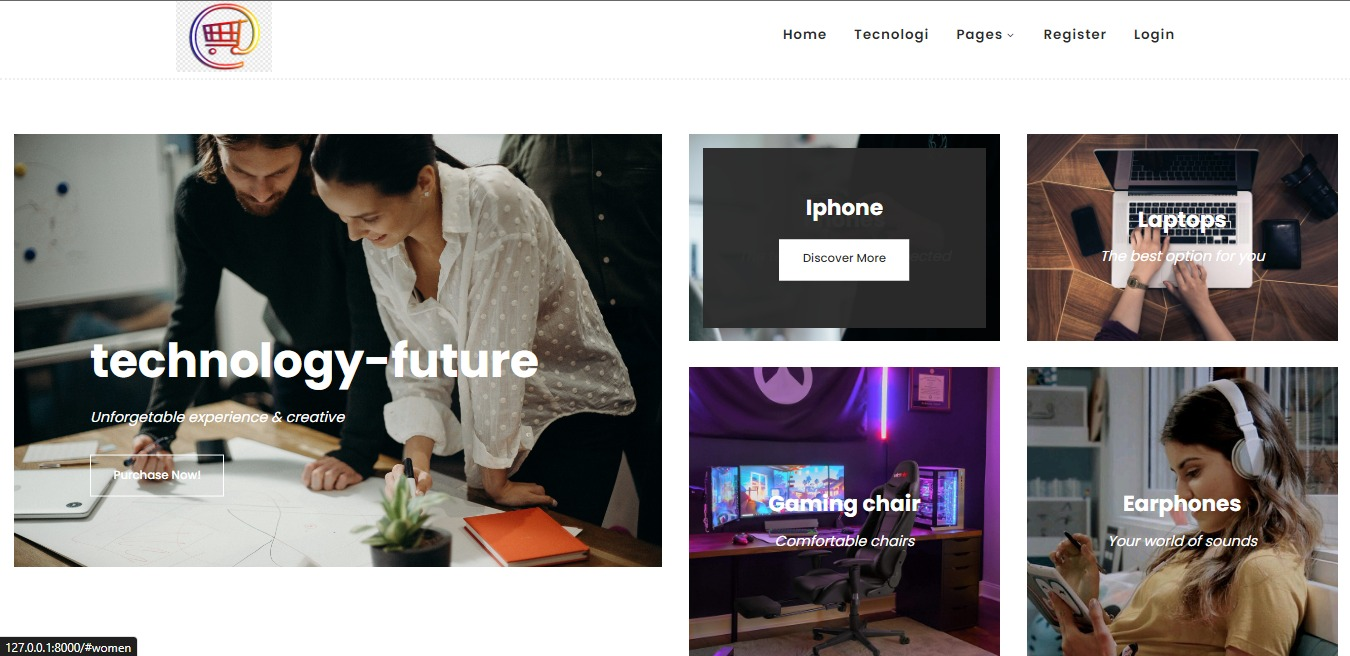
\includegraphics[width=0.8\textwidth,keepaspectratio]{img/imagen1.jpg}
	%\includesvg{img/automata.svg}
	%\label{img:mot2}
	%\caption{Product backlog.}
\end{figure}
\begin{figure}[H]
	\centering
	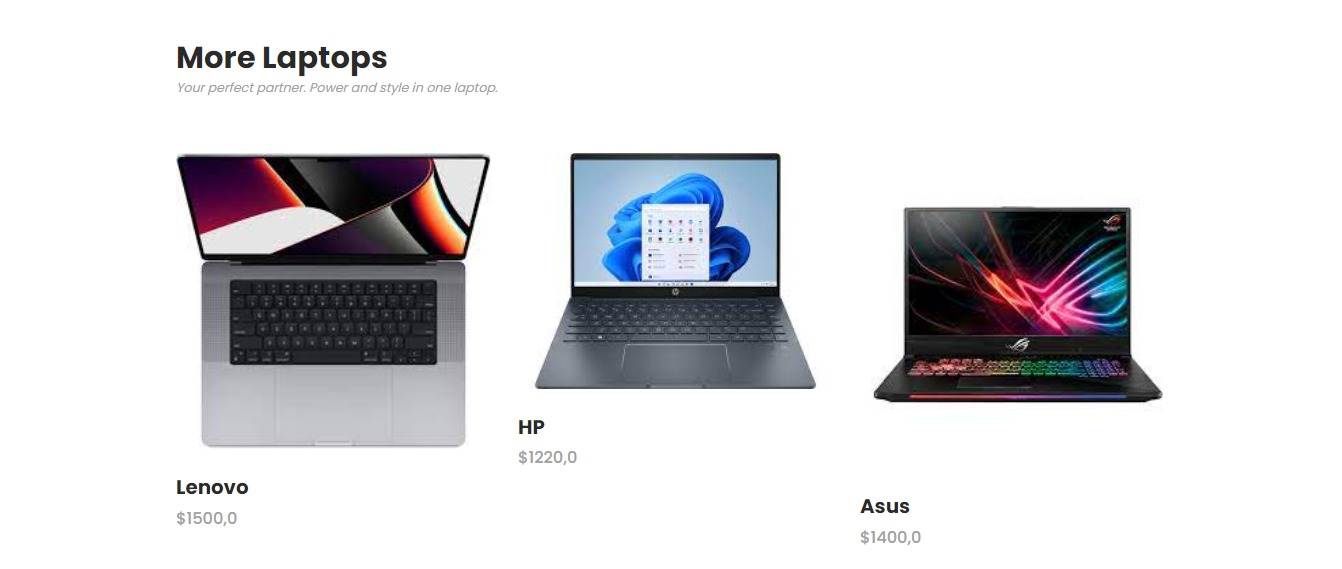
\includegraphics[width=0.8\textwidth,keepaspectratio]{img/imagen2.jpg}
	%\includesvg{img/automata.svg}
	%\label{img:mot2}
	%\caption{Product backlog.}
\end{figure}
\begin{figure}[H]
	\centering
	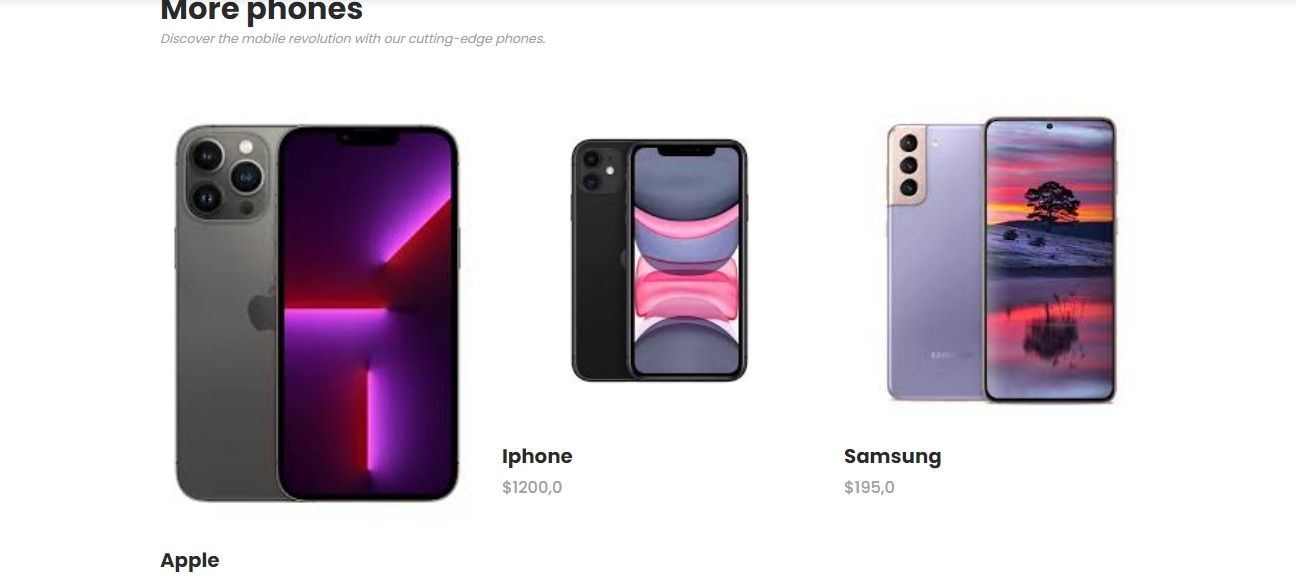
\includegraphics[width=0.8\textwidth,keepaspectratio]{img/imagen3.jpg}
	%\includesvg{img/automata.svg}
	%\label{img:mot2}
	%\caption{Product backlog.}
\end{figure}
\begin{figure}[H]
	\centering
	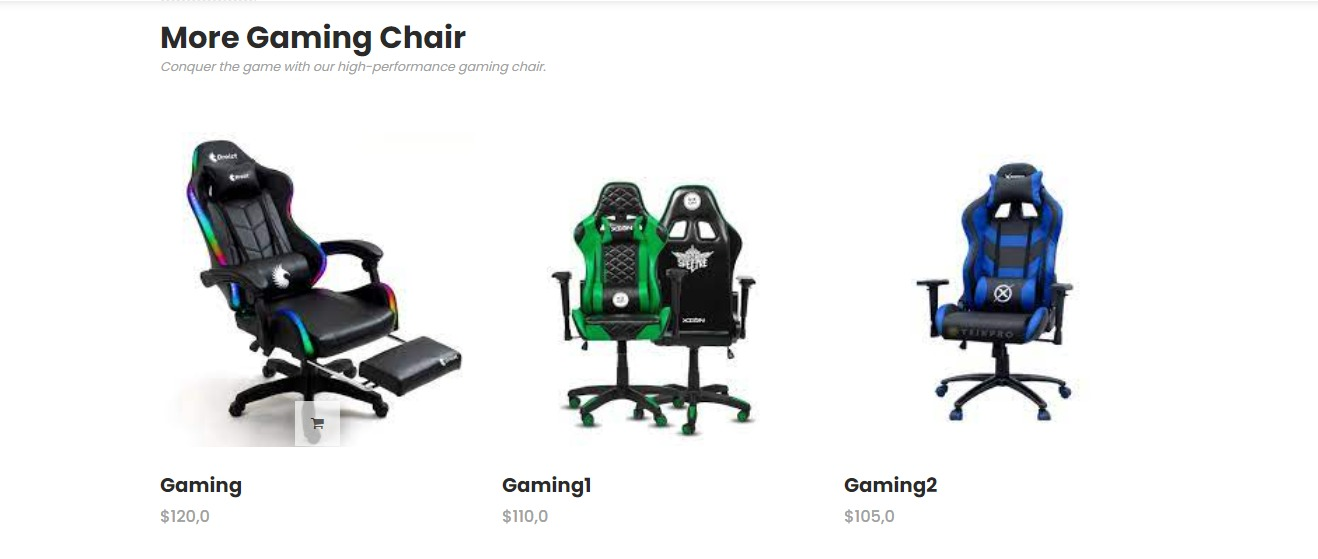
\includegraphics[width=0.8\textwidth,keepaspectratio]{img/imagen4.jpg}
	%\includesvg{img/automata.svg}
	%\label{img:mot2}
	%\caption{Product backlog.}
\end{figure}
\begin{itemize}	
	\item Register:
\end{itemize}	
\begin{figure}[H]
	\centering
	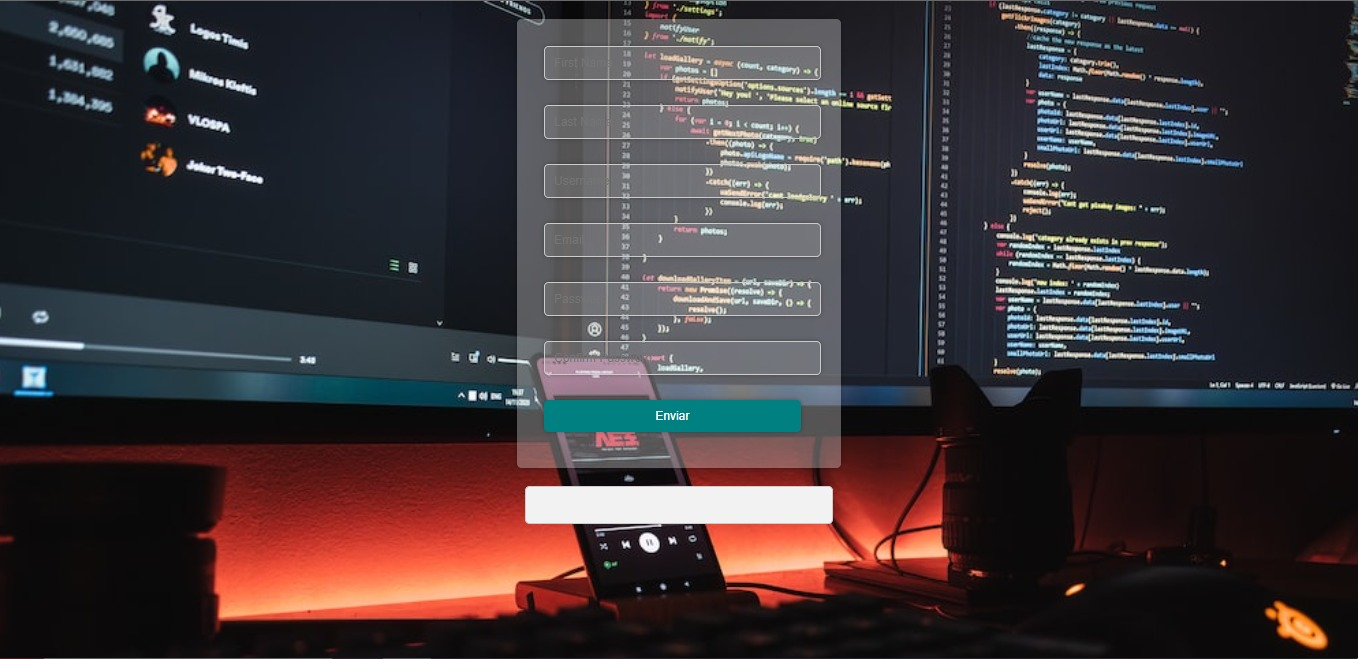
\includegraphics[width=0.8\textwidth,keepaspectratio]{img/imagen5.jpg}
	%\includesvg{img/automata.svg}
	%\label{img:mot2}
	%\caption{Product backlog.}
\end{figure}
\begin{itemize}	
	\item Login:
\end{itemize}	
\begin{figure}[H]
	\centering
	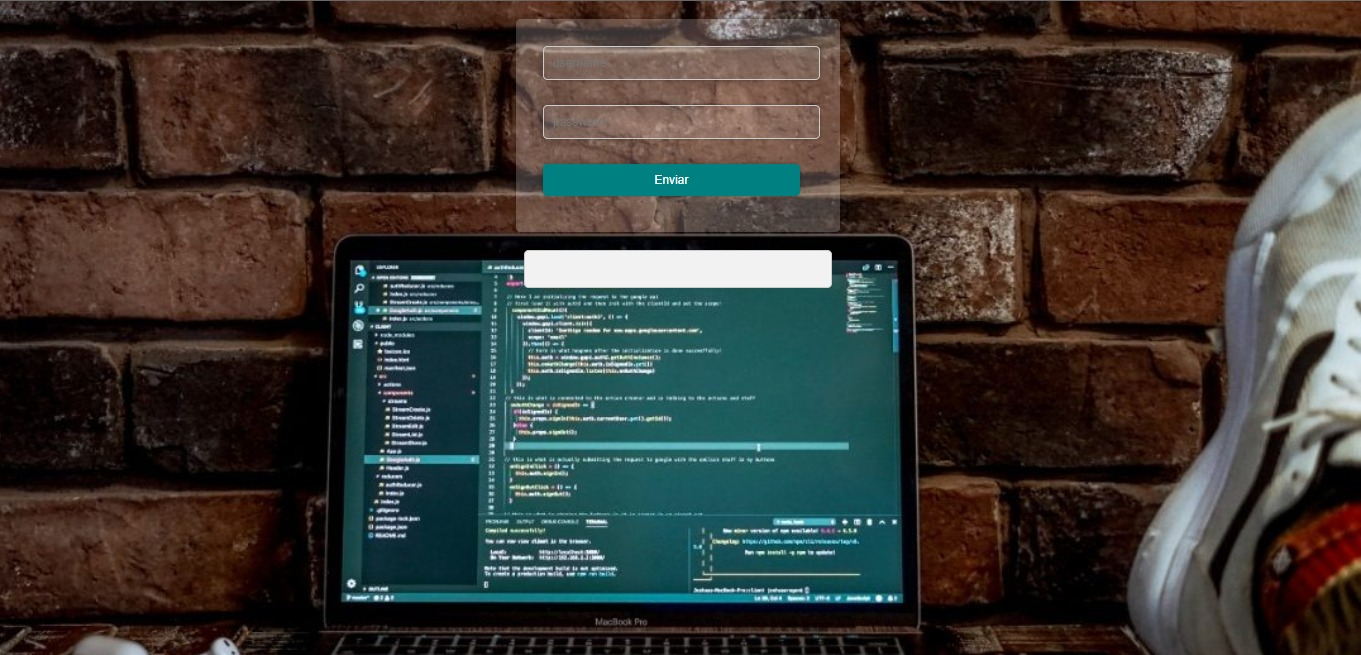
\includegraphics[width=0.8\textwidth,keepaspectratio]{img/imagen6.jpg}
	%\includesvg{img/automata.svg}
	%\label{img:mot2}
	%\caption{Product backlog.}
\end{figure}
\begin{itemize}	
	\item Base de datos:
\end{itemize}
\begin{figure}[H]
	\centering
	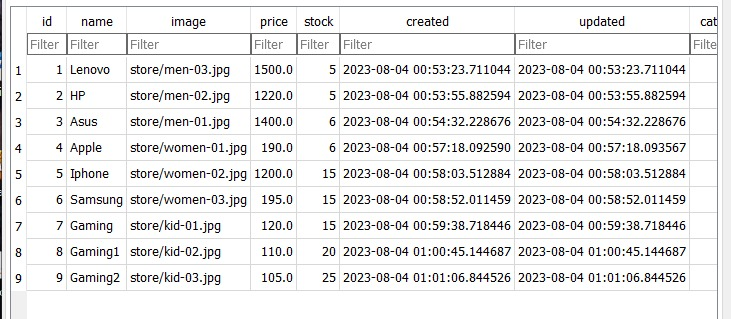
\includegraphics[width=0.8\textwidth,keepaspectratio]{img/imagen7.jpg}
	%\includesvg{img/automata.svg}
	%\label{img:mot2}
	%\caption{Product backlog.}
\end{figure}
\begin{figure}[H]
	\centering
	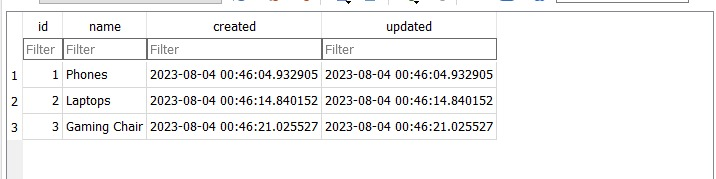
\includegraphics[width=0.8\textwidth,keepaspectratio]{img/imagen8.jpg}
	%\includesvg{img/automata.svg}
	%\label{img:mot2}
	%\caption{Product backlog.}
\end{figure}
\begin{figure}[H]
	\centering
	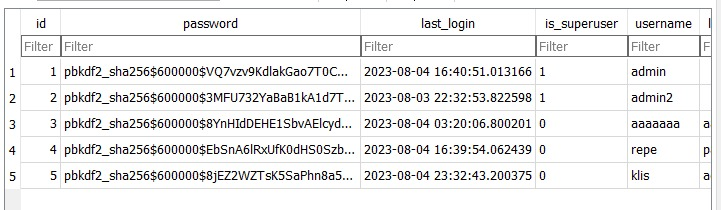
\includegraphics[width=0.8\textwidth,keepaspectratio]{img/imagen9.jpg}
	%\includesvg{img/automata.svg}
	%\label{img:mot2}
	%\caption{Product backlog.}
\end{figure}
\begin{figure}[H]
	\centering
	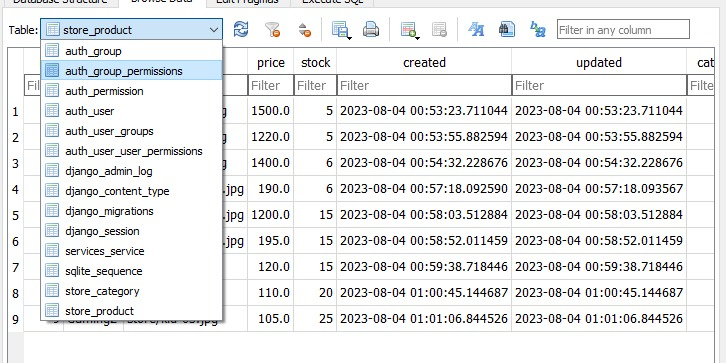
\includegraphics[width=0.8\textwidth,keepaspectratio]{img/imagen10.jpg}
	%\includesvg{img/automata.svg}
	%\label{img:mot2}
	%\caption{Product backlog.}
\end{figure}
\subsection{Estructura de laboratorio 09 - Proyecto Final}
\begin{itemize}	
	\item El contenido que se entrega del informe del laboratorio 09 - Proyecto Final es el siguiente:
\end{itemize}

\begin{lstlisting}[style=ascii-tree]
	Lab09-Informe/
   |--- informe-latex
	|--- contenido
   |   |--- actividades.tex
   |   |--- caratula.tex
   |   |--- github.tex
   |   |--- materiales.tex
   |   |--- preguntas.tex
   |   |--- referencia.tex
   |   |--- rubrica.tex
   |   |--- tarea.tex
	|--- img
   |   |--- logo_abet.png
   |   |--- logo_episunsa.png
   |   |--- imagen1.jpg
   |   |--- imagen2.jpg
   |   |--- imagen3.jpg
   |   |--- imagen4.jpg
   |   |--- imagen5.jpg
   |   |--- imagen6.jpg
   |   |--- imagen7.jpg
   |   |--- imagen8.jpg
   |   |--- imagen9.jpg
   |   |--- imagen10.jpg
   |   |--- imagen11.jpg
   |   |--- imagen12.jpg
   |--- src
   |    |--- admin.py
   |    |--- apps.py
   |    |--- cart.py
   |    |--- context_processor.py
   |    |--- forms.py
   |    |--- login.txt
   |    |--- models.py
   |    |--- register.txt
   |    |--- urls.py
   |    |--- views.py
   |--- pweb2_lab09_proyectofinal.pdf    
   |--- main.tex
\end{lstlisting}    

	\section{Pregunta: Como les fue con el trabajo del proyecto final?}
\begin{itemize}
	\item Fue un trabajo interesante para realizarlo con algunas dificultades, pero se pudo terminar. Realizando los objetivos que se pedian en la tarea.
\end{itemize}


	\section{\textcolor{red}{Rúbricas}}

\subsection{\textcolor{red}{Entregable Informe}}
\begin{table}[H]
	\caption{Tipo de Informe}
	\setlength{\tabcolsep}{0.5em} % for the horizontal padding
	{\renewcommand{\arraystretch}{1.5}% for the vertical padding
		\begin{tabular}{|p{3cm}|p{12cm}|}
			\hline
			\multicolumn{2}{|c|}{\textbf{\textcolor{red}{Informe}}}  \\
			\hline 
			\textbf{\textcolor{red}{Latex}} & \textcolor{blue}{El informe está en formato PDF desde Latex,  con un formato limpio (buena presentación) y facil de leer.}   \\ 
			\hline 
			
			
		\end{tabular}
	}
\end{table}

\subsection{\textcolor{red}{Rúbrica para el contenido del Informe y demostración}}
\begin{itemize}			
	\item El alumno debe marcar o dejar en blanco en celdas de la columna \textbf{Checklist} si cumplio con el ítem correspondiente.
	\item Si un alumno supera la fecha de entrega,  su calificación será sobre la nota mínima aprobada, siempre y cuando cumpla con todos lo items.
	\item El alumno debe autocalificarse en la columna \textbf{Estudiante} de acuerdo a la siguiente tabla:
	
	\begin{table}[ht]
		\caption{Niveles de desempeño}
		\begin{center}
			\begin{tabular}{ccccc}
				\hline
				& \multicolumn{4}{c}{Nivel}\\
				\cline{1-5}
				\textbf{Puntos} & Insatisfactorio 25\%& En Proceso 50\% & Satisfactorio 75\% & Sobresaliente 100\%\\
				\textbf{2.0}&0.5&1.0&1.5&2.0\\
				\textbf{4.0}&1.0&2.0&3.0&4.0\\
				\hline
			\end{tabular}
		\end{center}
	\end{table}	
	
\end{itemize}

\begin{table}[H]
	\caption{Rúbrica para contenido del Informe y demostración}
	\setlength{\tabcolsep}{0.5em} % for the horizontal padding
	{\renewcommand{\arraystretch}{1.5}% for the vertical padding
		%\begin{center}
		\begin{tabular}{|p{2.7cm}|p{7cm}|x{1.3cm}|p{1.2cm}|p{1.5cm}|p{1.1cm}|}
			\hline
			\multicolumn{2}{|c|}{Contenido y demostración} & Puntos & Checklist & Estudiante & Profesor\\
			\hline
			\textbf{1. GitHub} & Hay enlace URL activo del directorio para el  laboratorio hacia su repositorio GitHub con código fuente terminado y fácil de revisar. &2 &X &2 & \\ 
			\hline
			\textbf{2. Commits} &  Hay capturas de pantalla de los commits más importantes con sus explicaciones detalladas. (El profesor puede preguntar para refrendar calificación). &4 &X &2 & \\ 
			\hline 
			\textbf{3. Código fuente} &  Hay porciones de código fuente importantes con numeración y explicaciones detalladas de sus funciones. &2 &X &1 & \\ 
			\hline 
			\textbf{4. Ejecución} & Se incluyen ejecuciones/pruebas del código fuente  explicadas gradualmente. &2 &X &2 & \\ 
			\hline			
			\textbf{5. Pregunta} & Se responde con completitud a la pregunta formulada en la tarea.  (El profesor puede preguntar para refrendar calificación).  &2 &X &2 & \\ 
			\hline	
			\textbf{6. Fechas} & Las fechas de modificación del código fuente estan dentro de los plazos de fecha de entrega establecidos. &2 &X &2 & \\ 
			\hline 
			\textbf{7. Ortografía} & El documento no muestra errores ortográficos. &2 &X &2 & \\ 
			\hline 
			\textbf{8. Madurez} & El Informe muestra de manera general una evolución de la madurez del código fuente,  explicaciones puntuales pero precisas y un acabado impecable.   (El profesor puede preguntar para refrendar calificación).  &4 &X &3 & \\ 
			\hline
			\multicolumn{2}{|c|}{\textbf{Total}} &20 & &16 & \\ 
			\hline
		\end{tabular}
		%\end{center}
		%\label{tab:multicol}
	}
\end{table}

\clearpage
	
	\section{Referencias}
\begin{itemize}			
	\item \url{https://www.w3schools.com/python/python_reference.asp}
        \item \url{https://docs.djangoproject.com/en/4.2/howto/outputting-pdf/}
        \item\url{https://www.scaler.com/topics/django/relationships-in-django-models/}
        \item\url{https://docs.djangoproject.com/en/4.2/topics/email/}
\end{itemize}	
			
\end{document}